\documentclass[a4paper, 12pt]{article}
\usepackage[utf8]{inputenc}
\usepackage[T1]{fontenc}
\usepackage[french]{babel}
\usepackage{graphicx}
\usepackage{amsmath}
\usepackage{hyperref}
\usepackage{lmodern}
\usepackage{moreverb}
\usepackage{multicol}

\hypersetup{
    colorlinks=true,
    linkcolor=blue,
    filecolor=magenta,      
    urlcolor=cyan,
    pdftitle={Overleaf Example},
    pdfpagemode=FullScreen,
    }

\urlstyle{same}
\usepackage[a4paper,left=2cm,right=2cm,top=2cm,bottom=2cm]{geometry}

\pagestyle{headings}
\pagestyle{plain}


\setcounter{secnumdepth}{4}
\setcounter{tocdepth}{4}
\makeatletter


\makeatother



\makeatletter
\def\toclevel@subsubsubsection{4}
\def\toclevel@paragraph{5}
\def\toclevel@subparagraph{6}
\makeatother





\setlength{\parindent}{0cm}
\setlength{\parskip}{1ex plus 0.5ex minus 0.2ex}
\newcommand{\hsp}{\hspace{20pt}}
\newcommand{\HRule}{\rule{\linewidth}{0.5mm}}

\begin{document}

\begin{titlepage}
  \begin{sffamily}
  \begin{center}

   
    \textsc{\LARGE }\\[2cm]

    \textsc{\Large Compte rendu de Réunion}\\[1.5cm]
    \textsc{\Medium Rédigé par Ilyes ZEGHDALLOU}

    % Title
    \HRule \\[0.4cm]
    { \huge  \textsc{ StellaStone} \\
    \textsc{\Large By Novus}\\ [0.4cm] }
	

    \HRule \\[2cm]
    \textsc {Idriss BENGUEZZOU\\Mohammed ROUABAH\\Ghilas MEZIANE \\ Ilyes ZEGHDALLOU}
 \begin{figure}
     \centering
    
\includegraphics[scale=0.2]{logoUJM.png}
     \label{fig:ujm_logo}
 \end{figure}
   
    \

    \vfill

    % Bottom of the page
    {\large {} 10/10/2022}

  \end{center}
  \end{sffamily}
\end{titlepage}

\newpage

\section{Réunion du Vendredi 07/10}
La réunion de cette semaine à été tenue le 07/10. Celle-ci n'a malheureusement pas pu être tenue en présentiel, ce qui nous a contraint a créer un serveur Discord sur lequel nous avons pu créer différents salons : un salon pour chaque document demandé. Bien que la réunion ait été tenue en distanciel, tous les membres du groupe étaient 
présents, et celle ci s'est déroulée entre 19h et 20h.

 \begin{figure}[!h]
    \centering
    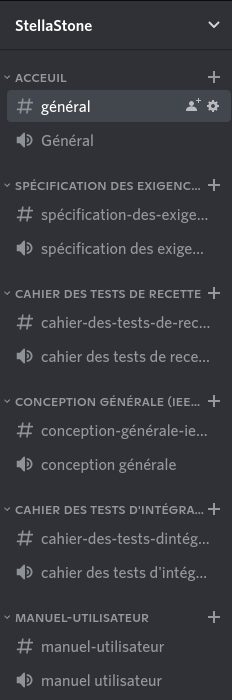
\includegraphics[scale=0.5]{discord.png}
    \label{fig:Le_planning}
    \caption{Capture d'écran du serveur DISCORD}
\end{figure}

\section{Un premier tour de table}

La réunion du jour avait donc pour premier objectif de vérifier l'avancement que l'on avait programmé pour cette semaine. Comme décidé lors de la précédente réunion, nos premiers objectifs ont été réalisés : \\
\begin{itemize}
    \item un repository git a été crée.
    \item un tableau Trello a été mis en place.
    \item un squelette word a été mis à disposition dans sur notre repository git pour servir de modèle à tous nos documents.\\
\end{itemize}

\newpage
Ensuite à tour de rôle, chaque membre a donné les informations qu'il a pu recueillir durant ses recherches de la semaine. \\Celles-ci portaient - pour certains - sur la fusée elle-même et son fonctionnement général, i.e quels sont les indispensables pour la construction d'une fusée, les contraintes qui s'imposent lors de sa construction et de son lancement dans l'espace. \\\\
D'autres ont recherché quels types de forces s'appliquent à une fusée lors de son décollage, dans l'espace et sur différentes planètes.
Beaucoup de vidéos, disponibles sur le web, nous ont permis de mieux comprendre les forces gravitationnelles.\\

Exemple : \href{https://www.lumni.fr/video/decollage-d-une-fusee-principe-d-action-et-reaction}{Décollage d'une fusée principe d'action et réaction}
 \\

Cette documentation nous a permis de découvrir un domaine que nous ne maîtrisons pas du tout et qui nous est étranger, étant informaticiens.\\ Ceci a soulevé un vif débat entre nous, certains voulaient se lancer directement dans la  rédaction du document de spécification des exigences en parallèle de la recherche d'informations générales sur le fonctionnement et le décollage d'une fusée, pendant que d'autres jugeaient nécessaire de se renseigner un maximum sur le sujet afin de vulgariser les concepts incontournables du domaine spatial, dans un souci de professionnalisme et de respect de la discipline.

Enfin chacun de nous a énuméré les exigences auxquelles il a pensé comme premier pas dans la rédaction du document de spécification des exigences. 


\section{Planification de la semaine}

 \begin{figure}[!h]
    \centering
    \includegraphics[scale=0.45]{trello.png}
    \label{fig:Tache_semaine}
    \caption{Planification de tâches sur Trello}
\end{figure}

Enfin nous avons décidé, suite à cette réunion, de rédiger nos comptes rendus de réunions sur l'outil Overleaf donc en Latex. Ce qui nous permet à tous d'avoir un accès collaboratif au document, de pouvoir le relire et le corriger, en temps réel. 

\newpage
\section{Mise à jour du diagramme de Gantt}

En dernier lieu, nous avons mis à jour le diagramme de Gantt que nous avions créé précédemment. Nous nous sommes mis d'accord sur des dates butoirs pour chaque document à rédiger comme premier calibrage. Ces dates sont susceptibles d'être avancées ou reculées en fonction de notre avancement. 
\\\\
 \begin{figure}[!h]
    \centering
    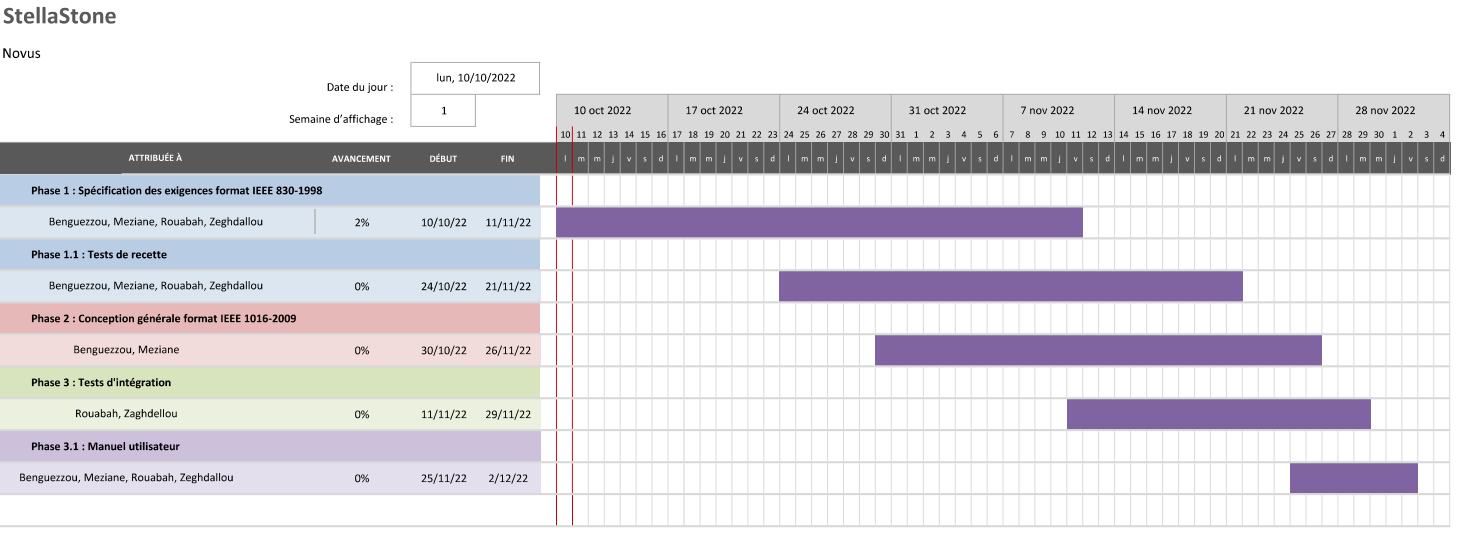
\includegraphics[scale=0.45]{Diagramme de gantt.png}
    \label{fig:Tache_semaine}
    \caption{Diagramme de Gantt}
\end{figure}

\end{document}